
\documentclass{standalone}
\usepackage[T1]{fontenc}
\usepackage[utf8]{inputenc}
\usepackage{pgf,tikz}

\begin{document}

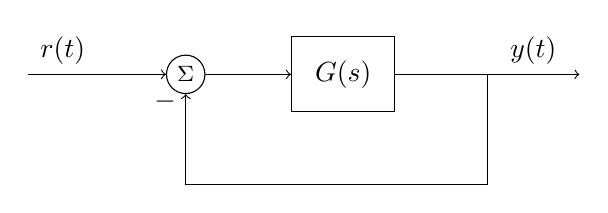
\begin{tikzpicture}[node distance=20mm, anchor=north]
  \node[coordinate] (input) {};
  \node[circle, draw, inner sep=2pt, right of=input] (sum) {\footnotesize $\Sigma$};
   \node[rectangle, draw, right of=sum, inner sep=3mm] (lti) {$G(s)$};
   \node[coordinate, right of=lti, node distance=30mm] (output) {};
   \draw[->] (input) -- node[near start, above] {$r(t)$}  (sum);
   \draw[->] (sum) -- node[near start, above] {}  (lti);
   \draw[->] (lti) -- node[coordinate] (meas) {} node[near end, above] {$y(t)$} (output);
   \draw[->] (meas) -- ++(0, -14mm) -| node[left, pos=0.96] {$-$} (sum);
 \end{tikzpicture}
\end{document}
